\documentclass[runningheads]{llncs}

\usepackage[T1]{fontenc}
\usepackage{graphicx}
\usepackage{amsmath,amssymb}
\usepackage{booktabs}
\usepackage{multirow}
\usepackage{xcolor}
\usepackage{listings}
\usepackage{tikz}
\usetikzlibrary{arrows.meta,positioning,shapes.geometric,fit,backgrounds}
\usepackage[hidelinks]{hyperref}
\usepackage{enumitem}
\usepackage{xspace}

% ---- tool-name macros ----
\newcommand{\tool}{\textsc{Dig-KN}\xspace}
\newcommand{\digold}{\textsc{Dig/SymInfer}\xspace}
\newcommand{\tvn}[1]{\textcolor{red}{[tvn: #1]}}

\lstset{basicstyle=\ttfamily\small,columns=fullflexible,keepspaces=true,
        mathescape=false,breaklines=true}
\definecolor{termbg}{RGB}{250,250,250}
\definecolor{termframe}{RGB}{210,215,220}
\definecolor{cmdcolor}{RGB}{0,50,150}
\definecolor{catcolor}{RGB}{130,30,30}
\definecolor{loccolor}{RGB}{0,100,100}
\lstdefinestyle{bashsession}{
    language=bash,
    basicstyle=\ttfamily\scriptsize,
    backgroundcolor=\color{termbg},
    frame=single,
    rulecolor=\color{termframe},
    keywordstyle=\color{cmdcolor}\bfseries,
    commentstyle=\color{gray!80!black}\itshape,
    stringstyle=\color{teal},
    showstringspaces=false,
    columns=fullflexible,
    keepspaces=true,
    breaklines=true,
    morekeywords={python3, dig, cohendiv},
    escapeinside={(*@}{@*)},
}
\newcommand{\code}[1]{\texttt{\small #1}}

\begin{document}

\title{\textsc{Dig-KN}: A Hybrid Tool for Generating and Proving Numerical Program Invariants}
%
\titlerunning{Dig-KN: A Hybrid Tool for Numerical Invariants}
%
\author{ThanhVu Nguyen\inst{1} \and
         Deepak Kapur\inst{2}\thanks{Deepak Kapur (1950--2026), co-creator of
         \textsc{Dig}, passed away during this work.  Kapur and Nguyen collaborated
         on dynamic and algebraic invariant generation across a series of works
         on polynomial, array, and disjunctive invariants~\cite{nguyen2009dig,nguyen2012dig,nguyen2014dig,nguyen2014tosem},
         and recently on making invariant generation accessible via automated web toolsets.
         \textsc{Dig-KN} is named in his honor and dedicated to his memory.}}
\authorrunning{Nguyen and Kapur}
\institute{George Mason University, USA \and
           University of New Mexico, USA\\
           \email{tvn@gmu.edu}}

\maketitle

\begin{abstract}
Numerical invariants---non-linear equalities, inequalities, congruences, and
min/max-plus disjunctions over program variables---underpin a wide
range of verification, complexity, and termination analyses.  We present
\tool{}, a hybrid tool that automatically generates such numerical invariants
at arbitrary program locations with zero manual configuration.  \tool{} descends from the \digold{} line of
symbolic-state invariant generators but is re-architected around three core pillars:
(i) a \emph{self-contained} symbolic-execution engine for C that eliminates external tool dependencies
and exposes sound reasoning primitives (symbolic-state constraint checking, ranking-function synthesis, termination/non-termination proofs, and targeted assertion verification);
(ii) dynamic \emph{finite-difference degree estimation} to automatically synthesize expressive non-linear polynomial relations without combinatorial term explosion; and
(iii) an integrated numerical inference pipeline combining dynamic equality fitting, octagonal inequality optimization, modular congruences, and min/max-plus disjunctions.
Complementary opt-in modules provide static algebraic ideal solving, shared-model optimization, and neural candidate proposal.
\tool{} uses seeded experiments and solver work-unit budgets, with wall-clock safeguards for expensive queries, and provides an interactive web interface at \url{https://dig.roars.dev}.  \tool{} is open source at \url{https://github.com/dynaroars/dig}.
\keywords{Program invariants \and Numerical invariants \and Dynamic analysis
\and Symbolic execution \and SMT optimization \and Static analysis.}
\end{abstract}

% =====================================================================
\section{Introduction}
\label{sec:intro}

Program invariants---logical relations over program variables that hold at a
given location on every execution---are central to software verification,
program understanding and reasoning\tvn{citations, see TSE paper}.
An important class of program invariants is \emph{numerical invariants}, which capture relations over numerical program variables: 
(non)linear equalities such as $q y + r = x$ and $y^2 - 2x + y = 0$, linear inequalities such as
$-x-y\le 10$, congruences such as $x \equiv 0 \pmod 4$, and disjunctive
relations captured in min/max-plus form such as $\max(x,y)\le z{+}2$.

The major paradigm for inferring such invariants is
\emph{counterexample-guided invariant generation} (CEGIR): cheaply
\emph{guess} candidate invariants (e.g., from concrete program states or traces, then
\emph{check} them and use counterexamples to refine, iterating to a fixpoint.
Our prior work, \digold~\cite{nguyen2021using,nguyen2017syminfer}, showed that
using \emph{symbolic program states}---compact encodings of large sets of
concrete states obtained from a symbolic executor---as the basis for checking
substantially improves the quality of inferred invariants and enables rich
forms (nonlinear equalities, octagonal inequalities, and min/max-plus
disjunctions).
That work, however, suffered from three fundamental limitations:
(i) it lacks of a way to infer polynomial growth degrees from traces, forcing users to either manually specify a degree ceiling or accept a combinatorial explosion of terms in high-degree templates; (ii) it is essentially a command-line tool that depends on external symbolic executors and SMT solvers, which are brittle to install and configure; and (iii) it does not guarantee soundness of the inferred invariants as the symbolic executor may not explore all feasible states.

This paper presents \tool{}, a complete re-engineering of the \digold{} line into a self-contained, fully automatic hybrid tool.  \tool{} reorganizes invariant synthesis around a built-in symbolic-execution engine that serves both as a shared \emph{basis} for inference and as a \emph{sound verification oracle}.  By default, \tool{} infers every numerical invariant family at an automatically predicted degree with zero configuration.  Concretely, our contributions are:

\begin{enumerate}[leftmargin=1.5em,itemsep=2pt]
\item A \textbf{self-contained symbolic-execution engine} for C (\S\ref{sec:arch}) that replaces external executors, produces symbolic states in-process without serialization overhead, bounds solver effort via a work-unit budget (\code{rlimit}) and wall-clock safeguards, and exposes sound verification primitives: constraint implication checking, ranking-function synthesis, and termination/non-termination proofs.
\item \textbf{Dynamic finite-difference degree estimation} (\S\ref{sec:degree}): a discrete finite-difference estimator that discovers the empirical polynomial growth order per variable from execution traces, guiding search to discover expressive non-linear equalities without combinatorial term explosion.
\item \textbf{Multi-domain numerical inference} (\S\ref{sec:inference}): an automated pipeline combining CEGIR polynomial equality fitting, direct SMT optimization for inequalities and min/max-plus disjunctions, and modular congruence synthesis.
\item \textbf{Sound verification core} (\S\ref{sec:verify}): built-in symbolic-state constraint checking to refine dynamic candidates and generate CEGIR counterexamples, combined with downstream property verification for safety assertions and loop termination.
\item \textbf{Downstream analysis applications} (\S\ref{sec:rq3}): demonstrations of \tool{} across program understanding, closed-form algorithmic complexity bounds, and termination/non-termination proofs.
\item An \textbf{interactive web interface} (\S\ref{sec:web}) for running \tool{} directly in the browser with containerized Docker sandboxing.
\end{enumerate}

\medskip\noindent\textbf{Target Audience and Intended Users.}
\tool{} is designed for: (i)~\emph{program verification and synthesis researchers} requiring sound, non-linear loop invariants and machine-checkable inductive certificates without brittle external toolchains; (ii)~\emph{software engineers and analysts} investigating unannotated or legacy numerical algorithms, discovering formal loop pre/post-specifications, or proving worst-case complexity and termination; and (iii)~\emph{educators and students} exploring formal methods, algebraic invariant ideals, and inductive verification interactively via the zero-install web interface.

% =====================================================================
\section{Overview and Architecture}
\label{sec:overview}

\subsection{Numerical Invariants and Symbolic States}
\label{sec:problem}
Let $L$ be a program location (e.g., a loop head annotated with \code{vtraceN(...)}).  A \emph{concrete $L$-state} maps the program variables in scope at $L$ to numerical values, and an invariant is a logical formula that holds over \emph{all} reachable concrete $L$-states.  Following~\cite{nguyen2021using}, a \emph{symbolic $L$-state} is a pair $\langle\sigma_L,\Pi_L\rangle$ where $\sigma_L$ maps variables to symbolic expressions over program inputs and $\Pi_L$ is a path condition; it denotes the (potentially unbounded) set of feasible concrete states reaching $L$.

\tool{} infers numerical invariants over several expressive template families:
\begin{itemize}[leftmargin=1.5em,itemsep=2pt]
\item \emph{Polynomial equalities:} $c_1 t_1 + \dots + c_n t_n = 0$ over monomial terms $t_i$ up to degree $d$ (e.g., $q\cdot y + r - x = 0$ or $y^2 - 2x + y = 0$).
\item \emph{Linear and octagonal inequalities:} $\pm x \pm y \le c$ and interval bounds (e.g., $-r \le 0, b - x \le 0$).
\item \emph{Min/max-plus disjunctions:} $\max(x, y) \le z + c$ or $\min(x, y) \le z + c$.
\item \emph{Modular congruences and arrays:} $t \equiv b \pmod n$ and array relations $A[i] = B[C[k\cdot i + c]]$.
\end{itemize}
An invariant is validated when it is verified over all reachable symbolic execution states $\Pi_L \implies p(\sigma_L)$, with spurious candidates eliminated through SMT counterexample generation and redundancy simplification.

\subsection{System Architecture and Self-Contained Symbolic Execution}
\label{sec:arch}
Fig.~\ref{fig:overview} depicts the architecture of \tool{}.  The central engineering decision in \tool{} is to \emph{build the symbolic executor from scratch} rather than depend on external tools (e.g., CIVL~\cite{siegel2015civl} or SPF~\cite{pasareanu2010spf}).

\begin{figure}[t]
\centering
\resizebox{0.95\textwidth}{!}{%
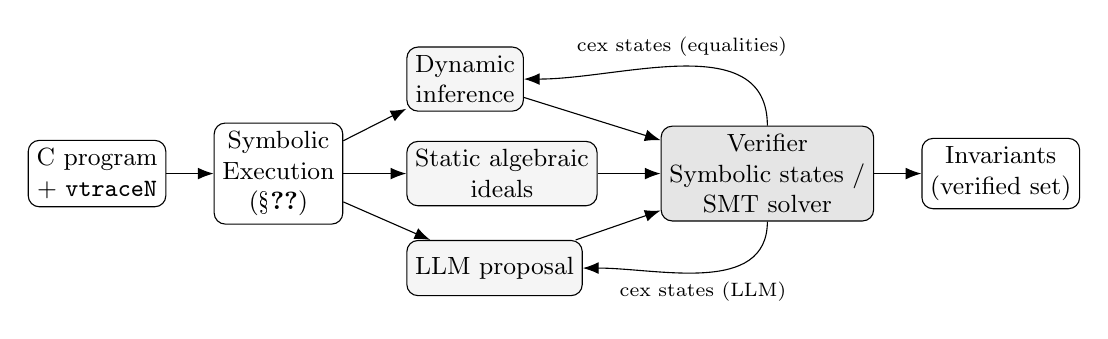
\begin{tikzpicture}[
   font=\small,
   box/.style={draw,rounded corners,align=center,minimum height=7mm,inner sep=3pt},
   eng/.style={box,fill=gray!8},
   core/.style={box,fill=gray!20},
   >={Latex[length=2mm]}]
 \node[box] (src) {C program\\+ \code{vtraceN}};
 \node[box,right=6mm of src] (se) {Symbolic\\Execution\\(\S\ref{sec:arch})};
 \node[eng,right=8mm of se,yshift=12mm] (dyn) {Dynamic\\inference};
 \node[eng,right=8mm of se] (stat) {Static algebraic\\ideals};
 \node[eng,right=8mm of se,yshift=-12mm] (llm) {LLM proposal};
 \node[core,right=8mm of stat] (ver) {Verifier\\Symbolic states /\\SMT solver};
 \node[box,right=6mm of ver] (out) {Invariants\\(verified set)};
 \draw[->] (src) -- (se);
 \draw[->] (se) -- (dyn); \draw[->] (se) -- (stat); \draw[->] (se) -- (llm);
 \draw[->] (dyn) -- (ver); \draw[->] (stat) -- (ver); \draw[->] (llm) -- (ver);
 \draw[->] (ver) -- (out);
 \draw[->] (ver.north) to[out=90,in=0] node[above,font=\scriptsize]{cex states (equalities)} (dyn.east);
 \draw[->] (ver.south) to[out=-90,in=0] node[below,font=\scriptsize]{cex states (LLM)} (llm.east);
\end{tikzpicture}%
}
\caption{\tool{} architecture.  A built-in symbolic execution engine feeds a portfolio of inference engines (\S\ref{sec:inference}), all validated by a unified symbolic-state verification core (\S\ref{sec:verify}).  Counterexample states refine CEGIR equality fitting and neural proposals; inequality maximization and static engines are one-shot.}
\label{fig:overview}
\end{figure}

The built-in engine parses a practical subset of C (integers, reals, conditionals, loops, 1D arrays, structs, globals, inlined functions) and explores paths up to a bounded unroll depth $D$, generating symbolic states $\langle\sigma_L, \Pi_L\rangle$ in-memory as Z3 ASTs with zero text serialization overhead.  Path feasibility uses a Z3 \emph{rlimit} (work-unit budget); wall-clock safeguards also bound expensive solver operations.  Seeded runs and recorded configurations support repeatability, but timeout decisions and internal parallel scheduling need not be identical across runs.  The engine exposes implication checking ($\Pi \Rightarrow p$), term maximization, ranking-function synthesis, and termination proofs.  Candidate validation over explored states is distinguished from separate unbounded inductive verification.

\subsection{A Worked Example: Inferring and Validating Invariants}
\label{sec:example}
To illustrate how the portfolio of inference engines and the verification core interact, we trace \tool{}'s execution on the geometric inner loop of an integer-division routine (\code{cohendiv.c}). Its loop head observes \code{q, r, a, b, x, y}, with loop body:
\begin{center}
\code{a = 1;\ b = y;\ while (r >= 2*b) \{ a = 2*a;\ b = 2*b; \}}
\end{center}
When invoked from either the command line (Fig.~\ref{fig:run}) or the web interface (Fig.~\ref{fig:web_ui}), \tool{} operates in four automated stages:

\medskip\noindent\textbf{1. Data-Driven Equality Fitting (\S\ref{sec:inference}).}
\tool{} instantiates a degree-$d$ template $\sum_i c_i t_i = 0$ over monomials $t_i$ in $\{a, b, y, a\cdot y, b\cdot y, \dots\}$. It evaluates concrete valuations sampled from symbolic states and solves the linear system for its null space, discovering basis vectors such as $a\cdot y - b = 0$ and $q\cdot y + r - x = 0$. Each candidate is checked against symbolic states; failing checks yield concrete counterexamples added as new rows to the matrix (the CEGIR loop).

\medskip\noindent\textbf{2. Algebraic Ideal Solving (\S\ref{sec:static}).}
When enabled (\code{-dokapur}), the algebraic ideal engine computes the same equality $a\cdot y - b = 0$ directly from the loop transition $a' = 2a, b' = 2b$ via the Rodr\'iguez-Carbonell--Kapur method without execution sampling.

\medskip\noindent\textbf{3. Multi-Domain Numerical Inference and Validation (\S\ref{sec:verify}).}
\tool{}'s inequality and min/max-plus engines infer companion bounds and relational constraints (e.g., $a\cdot y - b = 0$, $-r \le 0$, $-y \le -1$, $-a \le 0$). The symbolic verification core checks each candidate constraint against the collected symbolic path conditions ($\Pi_L \implies p(\sigma_L)$), pruning spurious relations and discharging valid invariants across explored paths.

\medskip\noindent\textbf{4. Post-Processing and Simplification.}
A post-processing pass simplifies redundant and weaker constraints via SMT implication (e.g., deduplicating algebraic and dynamic twins), emitting the minimal verified set.

% =====================================================================
\section{Numerical Invariant Inference Engines}
\label{sec:inference}

\subsection{Polynomial Equalities via CEGIR Null Space}
\label{sec:eqts}
For polynomial equality invariants, \tool{} parameterizes a template $\sum_{i=1}^M c_i t_i = 0$ over monomial terms $t_i$ over variables $\mathbf{x}$ up to degree bound $d$.  Concrete valuation vectors $\mathbf{v}^{(k)} \in \mathbb{Q}^M$ are drawn as models of reachable symbolic states.  Solving the linear system $V \mathbf{c} = \mathbf{0}$ via singular value / Gauss-Jordan decomposition yields a basis for the coefficient null space.

Each candidate equality is checked against the symbolic states $\langle\sigma_L, \Pi_L\rangle$.  If $\Pi_L \land \neg(p(\sigma_L))$ is satisfiable, SMT solver models provide concrete counterexample states that are appended as new rows to $V$, refining the null space.  Before symbolic checking, fitted equalities are tested against all collected concrete traces; diverse violating rows refine a basis that overfits early iterations.  The fitting basis is retained through refinement instead of discarding generators merely because their coefficients are large.  With an explicit degree ceiling, results at lower degrees are retained and all requested locations are searched even if an earlier pass found some equalities.  Gr\"obner simplification uses graded reverse lexicographic order and a bounded computation; on timeout, the original basis is preserved.

Counterexample replay distinguishes program-entry inputs from variables observed at trace locations.  Entry symbols use an \code{X\_} namespace, including model completion for unused inputs.  Replaying or excluding an input uses these entry values rather than a mutated variable's value at the observation point.  This distinction is essential on benchmarks such as \code{20.dig}, where confusing the two namespaces previously prevented useful concrete traces.

Concrete C executions are compiled with \code{-ftrapv}.  Signal-terminated executions, including any trace prefix printed before signed-integer overflow, contribute no samples.  This prevents machine-integer wraparound from contaminating inference intended to recover mathematical-integer relations; ordinary nonzero returns from \code{main} remain usable.

\subsection{Dynamic Finite-Difference Degree Estimation}
\label{sec:degree}
The template degree $d$ over $V$ variables requires solving a linear system with $\binom{V+d}{d}$ unknown coefficients.  Prior tools either fixed a global maximum degree ceiling (incurring severe combinatorial slowdowns on low-degree loops) or relied on static term budgets that under-guessed degrees on high-variable programs (forcing $d=1$ and missing non-linear invariants unless users manually passed \code{-maxdeg}).

\tool{} addresses this by dynamically estimating polynomial growth per location and variable as a heuristic search guide using discrete calculus over ordered iteration traces $(v_0, v_1, v_2, \dots)$ at loop heads.  By the fundamental theorem of finite differences, a variable $v_n$ evolves as a polynomial of degree $d$ in the loop counter if and only if its $d$-th forward difference $\Delta^d v_n$ is a non-zero constant (where $\Delta v_n = v_{n+1} - v_n$ and $\Delta^k v_n = \Delta^{k-1} v_{n+1} - \Delta^{k-1} v_n$).

\tool{} computes forward difference tables across initial loop iterations:
\begin{itemize}[leftmargin=1.5em,itemsep=2pt]
\item If $\Delta^d v_n = \text{const} \ne 0$ for sampled iterations, degree $d$ guides the empirical polynomial search degree.
\item On quadratic programs ($d=2$, e.g., \code{ps2}, \code{cav09\_fig2d}), finite differences confirm $d=2$, focusing search on compact 10-term quadratic bases (a 12$\times$ reduction over blind high-degree templates) and discovering quadratic equalities such as $y^2 - 2x + y = 0$ in $<1.5$\,s.
\item On cubic accumulators such as \code{cohencu}, degree hints guide search, but the growth degree need not equal the degree of a sufficient invariant basis.  In the recovery experiment, an explicit degree-2 search yields a basis implying $x=n^3$, $y=3n^2+3n+1$, and $z=6n+6$; the cubic target need not appear as a literal degree-3 generator.
\item On non-polynomial arithmetic (e.g., Euclidean subtraction in \code{egcd}), higher differences do not stabilize, and \tool{} avoids spurious high-degree template inflation.
\end{itemize}

\subsection{Inequalities, Min/Max-Plus, and Bound Optimization}
\label{sec:ineqs}
Unlike equalities, inequality inference in \tool{} is \emph{not} counterexample-guided; it uses direct SMT optimization.  For a candidate family of linear octagonal terms ($\pm x \pm y$), polynomial bounds, or min/max-plus operands ($\min(x,y), \max(x,y)$), \tool{} prunes trivially unbounded terms with a feasibility query and then \emph{maximizes} each term $t$ over the symbolic state space to obtain its provable upper bound $t \le c$.

The ordinary bound-search path uses satisfiability queries and binary search within a configured integer cap.  A bound is accepted only after checking that no larger feasible value exists; unknown, fractional, infeasible, unbounded, or out-of-cap results do not certify an optimum.  Optimization and redundancy queries have separate resource budgets.  When later concrete traces violate an inferred octagonal or min/max-plus bound, the bound may be weakened within the configured cap and retested; equalities are never weakened this way.  Domains execute sequentially so that each domain can use internal worker pools without nested daemon-process restrictions.  Candidate expressions are also projected through symbolic snapshot bindings before constraint checking, reducing queries that become identities.

\subsection{Modular Congruences and Array Relations}
\label{sec:congruences}
\tool{} infers modular congruences $t \equiv b \pmod n$ by computing the greatest common divisor (GCD) of successive trace differences $\gcd(\{v_{k+1} - v_k\})$, guarded against small-sample overfitting by testing against symbolic states.  For array-manipulating programs, \tool{} mines index relations $A[i] = B[C[k\cdot i + c]]$ across memory states.

\subsection{Additional Inference Capabilities}
\label{sec:additional_inf}
In addition to its default numerical inference pipeline, \tool{} implements three specialized, non-default inference engines:

\medskip\noindent\textbf{1. Static Algebraic Invariant Ideals (\code{-dokapur}).}
\label{sec:static}
Where loop updates follow deterministic straight-line polynomial transitions $\mathbf{x}' = T(\mathbf{x})$, \tool{} implements the Rodr\'iguez-Carbonell and Kapur bounded-degree ideal method~\cite{rodriguez2007kapur,rodriguez2007simple}. By analyzing polynomial orbits along loop transitions, it extracts the complete Gr\"obner basis of the invariant ideal in $<0.15$\,s with zero trace sampling.  A complete algorithmic formulation and limitation analysis is provided in Appendix~\ref{sec:appendix_kapur}.

\medskip\noindent\textbf{2. Shared-Model Optimization via \textsc{Symba} (\code{-dosymba}).}
\label{sec:symba_inf}
To optimize large pools of linear octagons and min/max-plus terms on high-variable programs, \tool{} implements simultaneous multi-objective SMT optimization via \textsc{Symba}~\cite{li2014symba}. Rather than issuing separate SMT queries for each term, \textsc{Symba} maintains a single shared solver instance, updating objective bounds from shared satisfying models and certifying all bounds optimal via a single \code{unsat} proof. Appendix~\ref{sec:appendix_symba} provides an extended analysis of \textsc{Symba}.

\medskip\noindent\textbf{3. Neural Invariant Proposal (\code{-llm}).}
\label{sec:llm}
For candidate generation beyond fixed algebraic or octagonal templates (e.g., complex piecewise conditionals, modular relations, or arbitrary non-linear inequalities), \tool{} integrates LLM prompting~\cite{pei2023llminv,kamath2023loopy,wu2024lemur} in a closed CEGIR loop. To evaluate an open foundation architecture while avoiding the drift and deprecation of closed proprietary APIs, our pipeline targets open-weight models---specifically the open-source \code{qwen/qwen3.8-27b} model from the Qwen family. In our experiments, we queried this model via Groq's cloud inference service rather than running it locally on our own GPU hardware; choosing an open-weight model ensures architectural transparency and allows users to self-host the same weights locally on-premise if desired.

The prompt explicitly provides the program source and execution traces sampled across loop locations, instructing the model to prioritize non-linear polynomial equalities ($p(x_1, \dots, x_n) = 0$, powers, and monomial products) as the primary focus while also proposing supporting inequalities, disjunctions, and closed forms. Crucially, all LLM proposals must pass \tool{}'s sound verification core (\S\ref{sec:verify}); the model is treated as an untrusted generator, and any candidate failing symbolic-state verification is immediately refuted with concrete counterexamples.

% =====================================================================
\section{Sound Verification Core}
\label{sec:verify}

The verification core provides sound reasoning infrastructure: candidate invariants mined from traces and algebraic templates are refined against symbolic path constraints, while integrated property provers verify downstream safety assertions and loop termination. In evaluation tables and reports, discovered invariants reflect constraints surviving symbolic verification, trace validation, and redundancy simplification.

\subsection{Symbolic-State Constraint Verification}
\label{sec:symbolic_ver}

The primary verification engine validates candidate invariants directly against the symbolic states $\langle\sigma_L, \Pi_L\rangle$ collected by the symbolic execution engine (\S\ref{sec:arch}):

\medskip\noindent\textbf{1. Constraint Implication Checking.}
For any candidate relation $p$ (e.g., a polynomial equality, octagon, or min/max disjunction), the verifier checks whether the path condition implies the property:
$$\Pi_L \implies p(\sigma_L)$$
If the implication holds across all feasible explored paths reaching $L$, the candidate is marked valid over the symbolic state space.

\medskip\noindent\textbf{2. Counterexample Extraction for CEGIR.}
If the negation $\Pi_L \land \neg p(\sigma_L)$ is $\code{sat}$, the SMT solver extracts a concrete input assignment that witnesses the violation. This concrete counterexample is either added as a new linear constraint to refine the CEGIR equality solver matrix (\S\ref{sec:eqts}) or returned to the LLM prompt (\S\ref{sec:llm}). Candidates that fail this check are marked \emph{disproved} and immediately discarded, filtering out spurious relations without manual intervention.

\medskip\noindent\textbf{3. SMT Redundancy Simplification.}
After inference engines emit candidate sets, \tool{} performs logical simplification via SMT implication. For each candidate $p \in \mathcal{C}$, the solver checks whether $\bigwedge (\mathcal{C} \setminus \{p\}) \implies p$. If valid, $p$ is logically redundant and pruned, ensuring the final emitted invariant set is compact.

\subsection{Target Property and Termination Verification}
\label{sec:additional_ver}

Beyond invariant synthesis, \tool{}'s verification core implements several specialized property-checking capabilities:

\medskip\noindent\textbf{1. Loop Termination via Invariant-Supported Ranking Functions.}
\tool{} automatically synthesizes linear ranking functions and lexicographic tuples $\langle R_1, \dots, R_m \rangle$. In isolation, ranking functions often fail decrease proofs under unconstrained havoc states; \tool{} feeds its inferred numerical invariants (e.g., $y \ge 1$) as inductive support lemmas to establish unbounded termination proofs.

\medskip\noindent\textbf{2. Non-Termination Proofs (\code{--nonterm}).}
For non-terminating loops, \tool{} synthesizes inductive recurrent sets (lassos), proving reachability from program entry and closure under the loop transition to formally certify infinite divergence.

\medskip\noindent\textbf{3. Targeted Assertion Verification (\code{--prove}).}
\tool{} allows verifying standalone user-specified assertions, safety invariants, and postconditions, automatically bundling auxiliary invariants to discharge inductive proofs.

% =====================================================================
\section{Tool Implementation and User Interfaces}
\label{sec:features}

\tool{} is implemented in Python and built on top of the Z3 SMT solver and \textsc{SymbC}, its internal symbolic execution and constraint verification engine for C programs.  \tool{} is architected for high-throughput parallel execution, taking full advantage of modern multi-core processors via Python multiprocessing: symbolic path exploration, concrete trace generation, candidate equality fitting across multiple program locations, and independent invariant verifications execute concurrently across forked worker processes.

\begin{table}[t]
\centering
\caption{\tool{} features and capabilities.}
\label{tab:features}
\small
\begin{tabular}{ll}
\toprule
\textbf{Aspect} & \textbf{Supported Features} \\
\midrule
Invariant types & Nonlinear/linear equalities, octagonal/polynomial \\
 & inequalities, min/max-plus disjunctions, congruences, arrays \\
Inference engines & Dynamic CEGIR equalities, direct SMT optimization, \\
 & RC--Kapur algebraic ideals (\code{-dokapur}), \\
 & \textsc{Symba} shared-model optimization, LLM proposal \\
Verification & Symbolic-state check, SMT implication, termination/ranking proofs \\
Symbolic execution & Built-in (C subset); deterministic Z3 \code{rlimit} \\
Degree estimation & Automatic per-location finite-difference prediction; \code{-maxdeg} cap \\
Interfaces & Command line, Python API, Docker container, web UI \\
\bottomrule
\end{tabular}
\end{table}

Tab.~\ref{tab:features} summarizes \tool{}'s features.  Several engineering design choices ensure practical reliability and seamless interaction across both local command-line and cloud browser workflows:

\subsection{Command-Line Interface and Execution}
\label{sec:cli}
On the command line, \tool{} is invoked directly as pure Python over Z3 and SymPy (Fig.~\ref{fig:run}):
\begin{center}
\code{python3 -O dig.py <benchmark.c>}
\end{center}
\tool{} is designed to be fully automatic and exceptionally easy to use, requiring little to no parameter tuning out of the box.  Its default configuration is robust, sane, and broadly applicable across diverse benchmark suites without manual intervention: \tool{} automatically estimates polynomial degrees via finite differences (\S\ref{sec:degree}), explores symbolic execution states, infers all supported numerical invariant families (non-linear equalities, octagonal inequalities, min/max-plus disjunctions, and congruences), and soundly validates candidates.  While \tool{} provides a rich suite of command-line options for specialized workflows---such as restricting invariant selectors via \code{-types eqt,ieq,\dots}, adjusting symbolic depth bounds, or toggling opt-in engines (\code{-dokapur}, \code{-dosymba}, \code{-llm})---the default settings are designed so that no parameter tweaking is necessary for standard usage.

\begin{figure}[t]
\begin{lstlisting}[style=bashsession]
(*@\textbf{\color{cmdcolor}\$\ python3\ -O\ dig.py\ cohendiv.c}@*)
* prog cohendiv locs 2; invs 25 (Eqt: 3, MMP: 1, Oct: 21) ...
-> time symbolic_states 0.3s, eqts 7.8s, ieqs 4.3s, minmax 21.0s, total 32.4s
(*@\textbf{\color{loccolor}vtrace1}@*) (11 invs):
  (*@\textbf{\color{catcolor}Eqt:}@*) q*y + r - x == 0
  (*@\textbf{\color{catcolor}Oct:}@*) -r <= 0; -q <= 0; -y <= -1; r - x <= 0; q - x <= 0; ...
  (*@\textbf{\color{catcolor}MinMax:}@*) min(q, y) - x <= 0
(*@\textbf{\color{loccolor}vtrace2}@*) (14 invs):
  (*@\textbf{\color{catcolor}Eqt:}@*) a*y - b == 0; q*y + r - x == 0
  (*@\textbf{\color{catcolor}Oct:}@*) -q <= 0; -y <= -1; -a <= -1; a - b <= 0; b - r <= 0; r - x <= 0; ...
\end{lstlisting}
\caption{\tool{} command-line interface session on \code{cohendiv.c} (output abridged).  Execution records configurations and validation outcomes.}
\label{fig:run}
\end{figure}

\subsection{The \tool{} Web Interface}
\label{sec:web}
To eliminate installation barriers, \tool{} provides an interactive web interface at \url{https://dig.roars.dev} (Fig.~\ref{fig:web_ui}).  The interface allows developers, researchers, and students, e.g., those interested in program analysis, formal verification, and invariant generation, to easily explore and experiment with \tool{} as well as its underlying \textsc{SymbC} engine directly in the browser.

The frontend is statically hosted on GitHub Pages, while a sandboxed backend executes user programs inside isolated Docker containers.  Users can select built-in benchmarks or paste custom C code and trace CSVs, configure numerical invariant families, inspect categorized invariant tables with live proved/candidate indicators, and exercise standalone $k$-induction, symbolic state exploration, and termination proofs without requiring any local tool installation.

\begin{figure}[htbp]
\centering
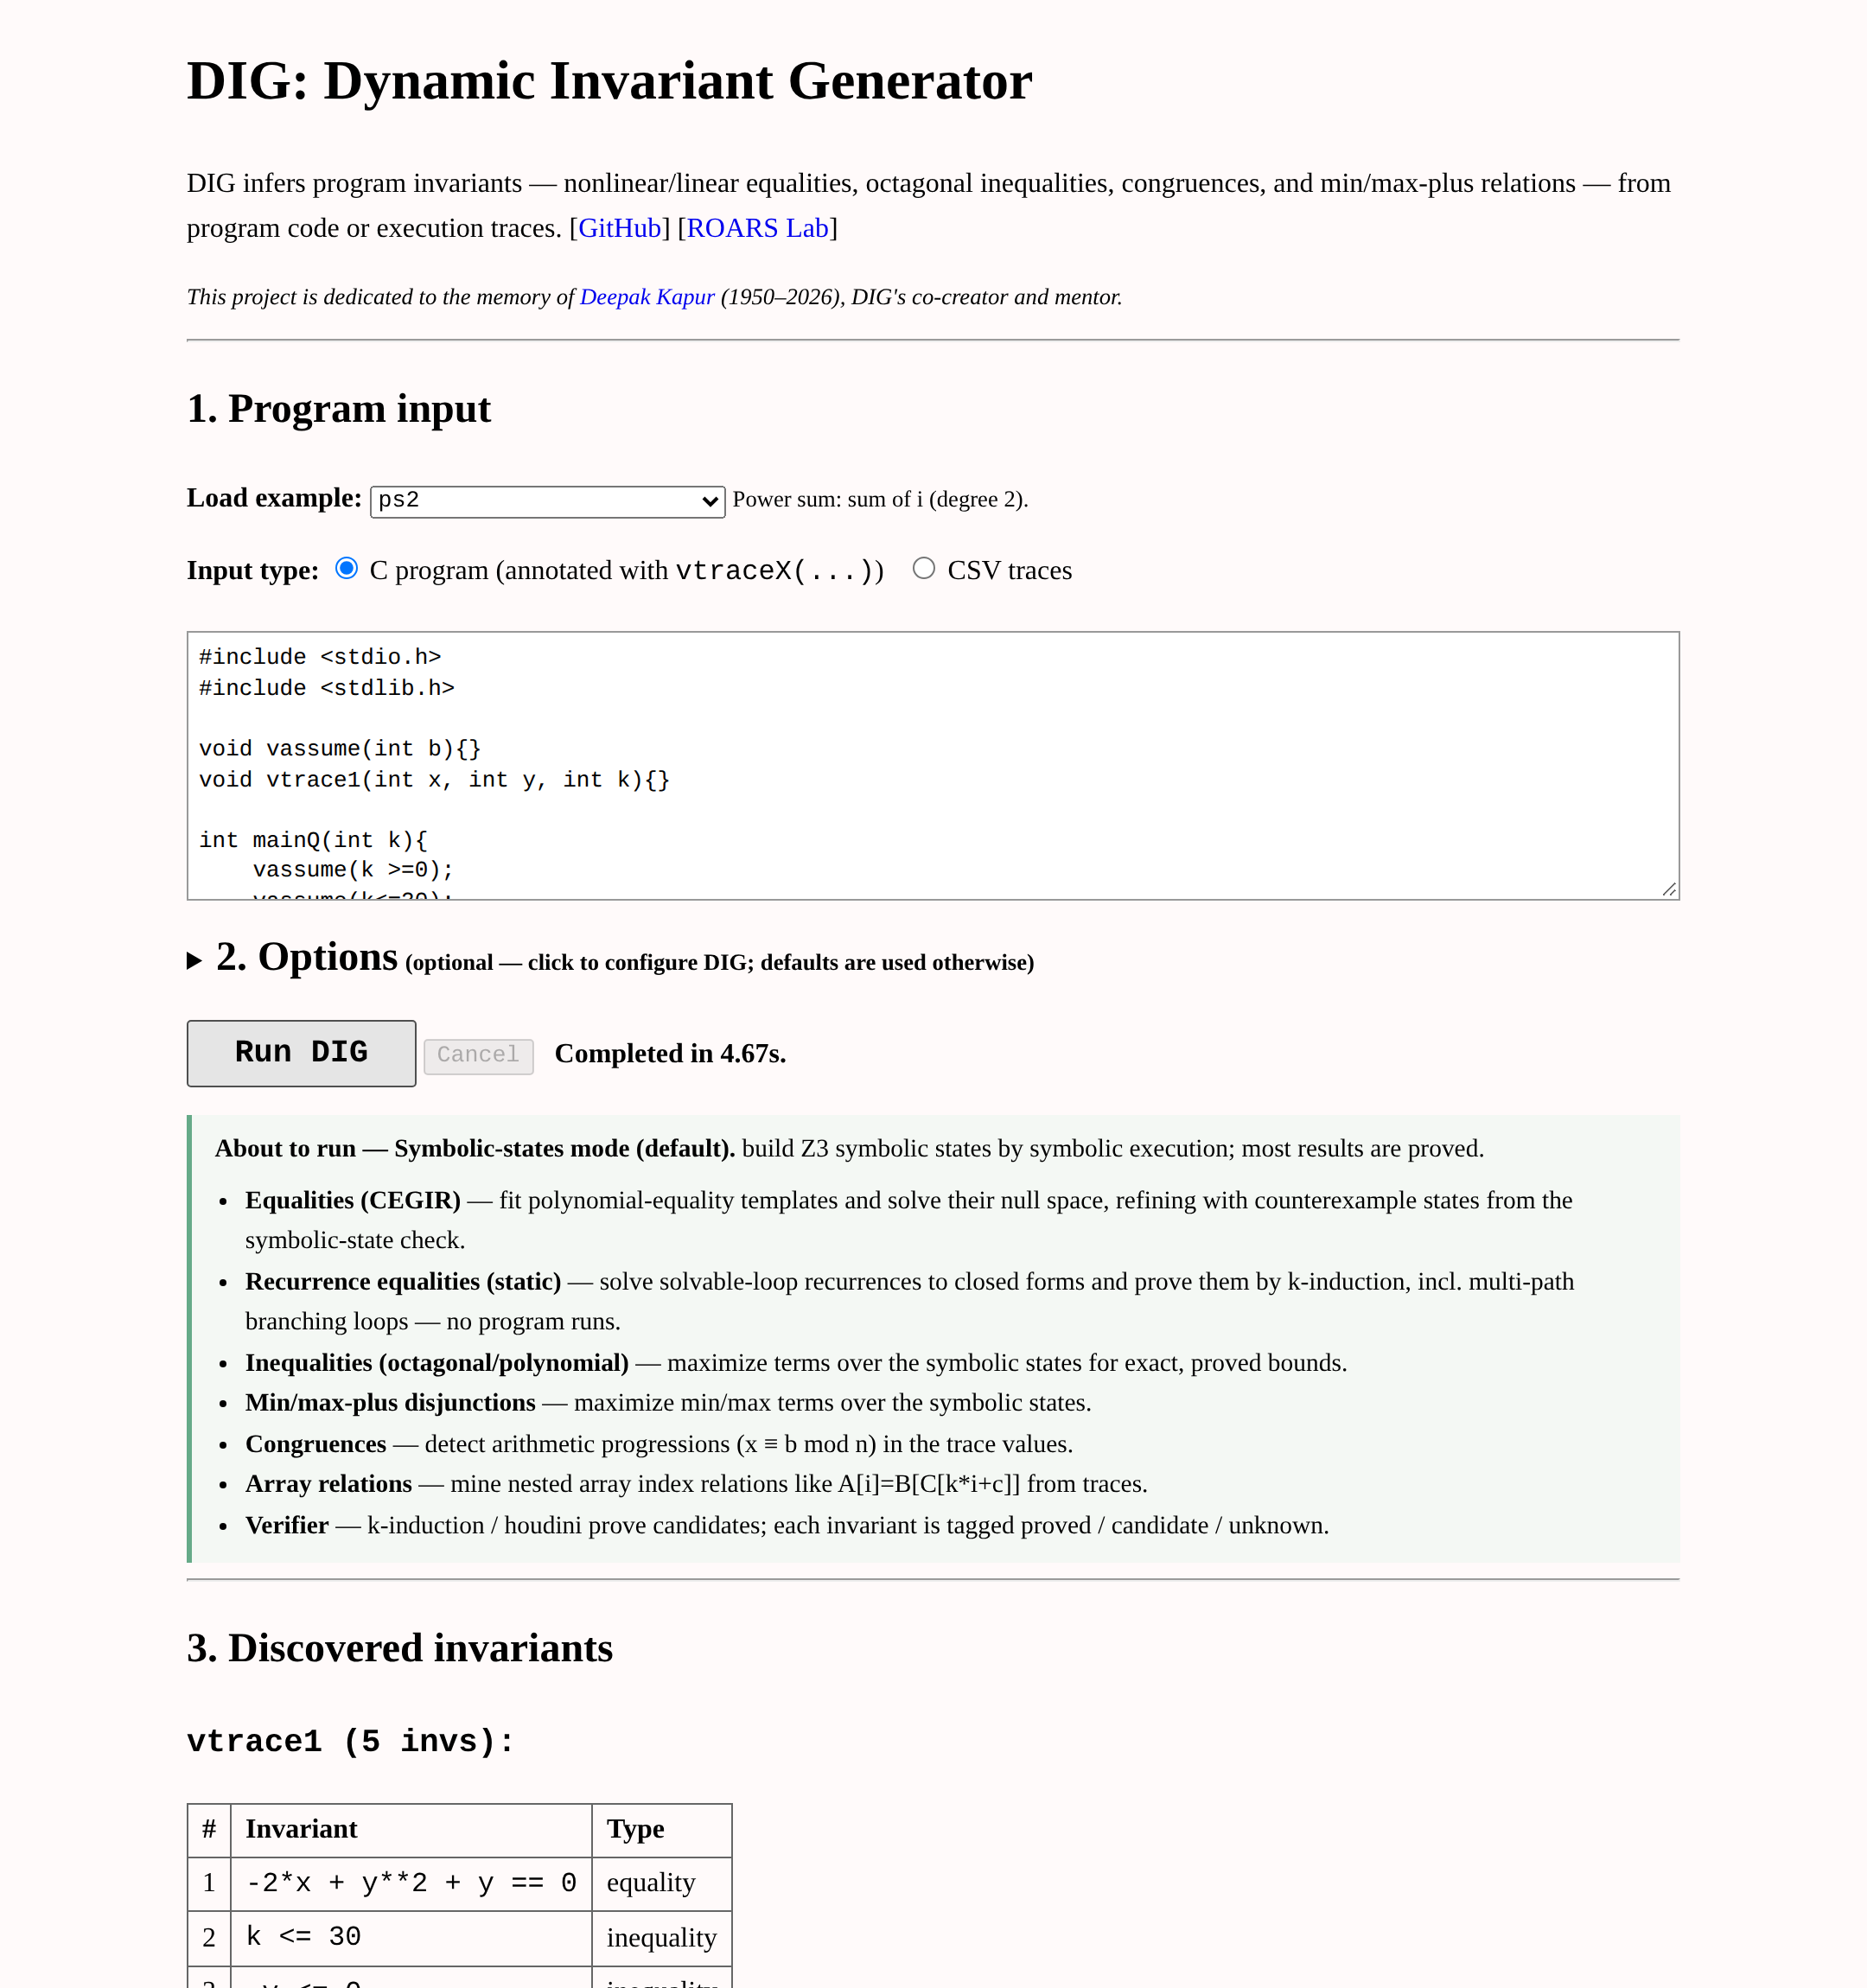
\includegraphics[width=0.85\textwidth]{web_ui.png}
\caption{\textsc{Dig-KN} interactive browser interface (\url{https://dig.roars.dev}) evaluating the quadratic power sum benchmark (\texttt{ps2.c}). The interface provides one-click example loading, configurable inference options, live containerized execution, and structured categorization of synthesized equalities ($y^2 - 2x + y = 0$) and inequalities ($-x \le 0, -y \le 0, y - x \le 0$) in the Discovered Invariants results table.}
\label{fig:web_ui}
\end{figure}

% =====================================================================
\section{Evaluation}
\label{sec:eval}

We evaluate \tool{} across four research questions:
inference effectiveness (\textbf{RQ1}),
the empirical impact and ablations of its core algorithmic features (\textbf{RQ2}),
applications of inferred invariants (\textbf{RQ3}),
and the effectiveness of using LLMs as a heuristic to infer candidate proposals (\textbf{RQ4}).\tvn{done}

\paragraph{Benchmarks}  We use three existing benchmark suites from \digold{}\cite{nguyen2021using} comprising 97 C programs.\tvn{done}

\begin{enumerate}[leftmargin=1.5em,itemsep=1pt]
  \item \textbf{NLA (33 programs):} This suites, which constitutes the \code{nla-digbench} categories in SV-COMP~\cite{svcomp,beyer2024svcomp},
        consist of programs implementing mathematical algorithms featuring multi-variable nonlinear polynomial equalities up to degree 5.\tvn{done}  

  \item \textbf{Complexity (19 programs):}
        Benchmark programs from Gulwani et al.~\cite{gulwani2009speed} instrumented with iteration counters to evaluate worst-case algorithmic complexity under nested loops, multi-phase dynamic resets, and alternating branches.\tvn{done}

  \item \textbf{HOLA (45 baseline programs):} Introduced by Dillig et al.~\cite{dillig2013hola}, these programs are designed to test inductive invariant generation under multi-path control flow and conditional branch updates.\tvn{done}
        
\end{enumerate}
% Among these suites, NLA is the primary mathematical stress test for nonlinear numerical invariant synthesis, demanding the discovery of high-degree polynomial ideals where monomial spaces grow combinatorially ($O(V^d)$) and SMT nonlinear integer arithmetic is notoriously hard.  Complexity requires deriving exact ranking relations and closed-form iteration bounds, while HOLA focuses on multi-path control-flow branching over small variable spaces ($V \le 4$).

\paragraph{Setup.}  Experiments were run on an Intel Core i7-7700
CPU (3.60\,GHz, 8 threads) with 32\,GB RAM running Linux.
Each benchmark program is run with a 600s timeout and runs 7 times to avoid accidental bias from random seeds.
We do not use any parameter tuning or manual configuration for the baseline evaluation, and all results are reported on the default configuration of \tool{}.
\tvn{done}


\subsection{RQ1: Effectiveness and Invariant Synthesis}
\label{sec:rq1}

How does the current \tool{} compare with the TSE'21 results?  Tab.~\ref{tab:comparison} reports the suite-level historical runtimes beside the new DIG timings and coverage. The timing comparison is descriptive rather than controlled: hardware, settings, and completed program populations differ. For invariant outputs, we count a TSE relation as matching when the new output implies it, even if the polynomial basis or expression differs; only cases without a certified implication are disagreements.

\begin{table}[t]
\centering
\caption{Uniform-configuration baseline campaign alongside historical \textsc{Dig/SymInfer} (TSE'21) timing references. DIG medians condition on completed runs; hardware and settings differ, so these are not controlled speedup measurements.}
\label{tab:comparison}
\begin{tabular}{lcccc}
\toprule
Suite & Programs Finished & Run Attempts & TSE'21 (s) & \tool{} (s) \\
\midrule
% BEGIN UNIFORM BASELINE PROGRESS
NLA & 6/33 & 44/231 & 73.1 & 7.83 \\
Complexity & 0/19 & 0/133 & 14.8 & -- \\
HOLA & 0/45 & 0/315 & 29.4 & -- \\
\textbf{Overall} & \textbf{6/97} & \textbf{44/679} & \textbf{38.2} & \textbf{7.83} \\
% END UNIFORM BASELINE PROGRESS
\bottomrule
\end{tabular}
\end{table}

The new DIG is evaluated with one shared configuration across all three suites. The campaign is still in progress; the table reports completed runs to date, and we will update it as each suite finishes. Invariant comparison is semantic: an output counts as agreeing with a TSE result if it implies the published relation, even when DIG expresses it in a different polynomial basis. We will discuss only cases that remain disagreements after this check.

% =====================================================================
\subsection{RQ2: Impact and Effectiveness of New Algorithmic Features}
\label{sec:rq2}

This question examines how the numerical inference engines contribute to the tool's results. The ablation below compares the full configuration with configurations that omit one domain. Across these nine evaluated cases, each configuration solved all benchmarks; removing domains reduced runtime in some cases, reflecting the cost of inference as well as its contribution to output breadth.

\begin{table}[t]
\centering
\caption{RQ2: ablation of numerical invariant inference engines across evaluated benchmarks. Reported times are mean wall-clock seconds across seven runs.}
\label{tab:rq3}
\begin{tabular}{lcc}
\toprule
Configuration & Solved & Time (s) \\
\midrule
Full \tool{} (all numerical domains) & 9/9 (100\%) & 14.23 \\
$-$ Min/Max-Plus Disjunctions & 9/9 (100\%) & 7.48 \\
$-$ Non-linear Equalities & 9/9 (100\%) & 9.71 \\
$-$ Inequalities / Octagons & 9/9 (100\%) & 12.53 \\
$-$ Congruences & 9/9 (100\%) & 13.80 \\
\bottomrule
\end{tabular}
\end{table}

The full system combines trace-based finite-difference degree estimation for polynomial search with symbolic-state checking and counterexample-guided refinement. The symbolic verifier rejects candidates that fit only the observed traces, while shared-model optimization supports bounds across large candidate sets. These components address different parts of the inference pipeline; the ablation measures domain-level effects, not the isolated causal effect of each algorithmic improvement.

\subsection{RQ3: Downstream Applications: Program Understanding, Complexity, and Termination}
\label{sec:rq3}

Inferred numerical invariants can provide specifications for unannotated programs and support downstream analyses. For example, the division relation $q y + r = x$ together with $0 \le r < y$ describes the quotient and remainder at the loop postcondition. On instrumented complexity benchmarks, relations between counters and inputs can expose iteration bounds and phase behavior. The tool also reuses inferred constraints in termination proofs: an invariant such as $y \ge 1$ can supply the missing precondition needed to prove that a division loop's remainder decreases. For a diverging loop, the optional recurrent-set engine can instead establish non-termination by finding a reachable set closed under the transition.

These examples illustrate how inferred constraints can serve as program explanations and proof support; they are separate from the suite-level runtime comparison in RQ1.

\subsection{RQ4: Neural Invariant Proposal and Soundness Verification}
\label{sec:rq4}

The optional neural proposer uses an open-weight Qwen model through Groq's inference API to suggest candidate equalities, inequalities, and disjunctions from program source and execution traces. The model is treated as an untrusted proposal source: every candidate is checked against symbolic states, and counterexamples are used to reject or refine candidates that do not hold. This lets the system use model-generated forms beyond its fixed numerical templates while retaining the same verification requirement as other inferred candidates. LLM proposals complement the systematic numerical engines; they do not replace them, particularly for tight bounds or branch-dependent relations.

% =====================================================================
\section{Related Work}
\label{sec:related}

\tool{} builds on dynamic invariant generation, from Daikon's template-based
mining~\cite{ernst2007daikon} to \textsc{DIG}'s polynomial and disjunctive
numerical candidates~\cite{nguyen2012dig,nguyen2014dig}. NumInv combined
numerical inference with symbolic execution and counterexample refinement
\cite{nguyen2017numinv}; \digold{} introduced symbolic-state-based inference
and checking~\cite{nguyen2021using,nguyen2017syminfer}. Its static algebraic
engine draws on polynomial ideal methods~\cite{rodriguez2007kapur,rodriguez2007simple,mullerolm2004,hrushovski2018},
while its inequality optimization builds on \textsc{Symba}~\cite{li2014symba}.

LLM-based invariant work spans direct invariant proposals~\cite{pei2023llminv,kamath2023loopy},
LLM-assisted verification~\cite{wu2024lemur}, and recent combinations with
bounded model checking~\cite{wu2024llmbmc,pirzada2024llmbmc} or
counterexample-guided clause assembly~\cite{cao2025clause2inv}. Earlier neural
inference includes G-CLN's learned nonlinear invariants~\cite{yao2020gcln};
goal-directed methods such as PIE and ICE also use learned predicates and
counterexamples~\cite{padhi2016pie,garg2016ice}. \tool{} combines dynamic,
static-algebraic, symbolic, and neural numerical-invariant generation in one
tool, with the LLM serving as an untrusted proposer behind its built-in
symbolic-state verifier.

% =====================================================================
\section{Conclusion and Future Work}
\label{sec:concl}

\tool{} turns the symbolic-state invariant-generation line into a self-contained
hybrid tool: a built-in symbolic executor that provides sound constraint
validation and counterexample generation, algebraic polynomial ideal solving, dynamic
finite-difference degree estimation, shared-model optimization, and optional neural
proposal---all behind a zero-configuration command line and a browser interface.
Future work includes Positivstellensatz/SOS nonlinear inequalities,
implication-counterexample (ICE) learning, a CHC back end, and a standalone
release of the symbolic-execution engine.

% \begin{credits}
% \subsubsection{\ackname}
% This material is based in part upon work supported by the National Science Foundation.
% 
% \subsubsection{Data Availability Statement.}
% \tool{} is open source at \url{https://github.com/dynaroars/dig} and usable without installation at \url{https://dig.roars.dev}.
% 
% \subsubsection{\discintname}
% The authors have no competing interests to declare that are relevant to the content of this article.
% \end{credits}

\bibliographystyle{splncs04}
\bibliography{refs}

\newpage
\appendix
\renewcommand{\thesection}{\Alph{section}}
\renewcommand{\theHsection}{\Alph{section}}
\renewcommand{\thesubsection}{\thesection.\arabic{subsection}}
\renewcommand{\theHsubsection}{\thesection.\arabic{subsection}}
\section{Detailed Benchmark Results}
\label{sec:appendix_benchmarks}

Tab.~\ref{tab:benchmarks_detail} retains representative outputs and timing summaries from the baseline campaign.  These entries predate the recovery fixes and benchmark alignment described below; they are not current-source target-recovery evidence.

\begin{table}[h!]
\centering
\caption{Baseline outputs of \tool{} on representative benchmarks ($L$: locations, $V$: max variables, $T$: total invariants, $E$: equalities, $I$: inequalities/octagons, $M$: min/max-plus, $C$: congruences, $NL(d)$: nonlinear invariants of max degree $d$). Reported metrics are medians across completed runs conditional on completion.}
\label{tab:benchmarks_detail}
\small
\setlength{\tabcolsep}{3.5pt}
\begin{tabular}{llccrcccccr}
\toprule
Suite & Benchmark & $L$ & $V$ & $T$ & $E$ & $I$ & $M$ & $C$ & $NL(d)$ & Time (s) \\
\midrule
\multirow{7}{*}{NLA} 
& \code{ps2}             & 1 & 3 & \textbf{5}  & 1 & 4  & 0 & 0 & 1 (2) & 8.35 \\
& \code{ps1}             & 1 & 3 & \textbf{5}  & 1 & 2  & 2 & 0 & --    & 7.47 \\
& \code{divbin}          & 2 & 5 & \textbf{15} & 3 & 9  & 3 & 0 & 1 (2) & 24.75 \\
& \code{sqrt1}           & 1 & 4 & \textbf{8}  & 2 & 4  & 0 & 2 & 3 (2) & 26.42 \\
& \code{geo1}            & 1 & 4 & \textbf{9}  & 1 & 6  & 1 & 1 & 1 (2) & 19.09 \\
& \code{hard}            & 2 & 6 & \textbf{23} & 5 & 12 & 4 & 2 & 5 (2) & 37.57 \\
& \code{mannadiv}        & 1 & 5 & \textbf{8}  & 1 & 7  & 0 & 0 & 1 (2) & 33.37 \\
\midrule
\multirow{7}{*}{NLA-mosaic}
& \code{fibonacci}               & 1 & 2 & \textbf{3}  & 1 & 2  & 0 & 0 & 1 (4) & 7.70 \\
& \code{fibonacci\_sign}         & 1 & 3 & \textbf{6}  & 2 & 4  & 0 & 0 & 2 (2) & 7.38 \\
& \code{pell}                    & 1 & 2 & \textbf{6}  & 1 & 2  & 0 & 3 & 1 (2) & 58.56 \\
& \code{chebyshev}               & 1 & 3 & \textbf{5}  & 0 & 2  & 3 & 0 & --    & 12.83 \\
& \code{welford}                 & 1 & 5 & \textbf{14} & 0 & 14 & 0 & 0 & --    & 20.97 \\
& \code{continued\_fract\_sign}  & 1 & 5 & \textbf{11} & 2 & 9  & 0 & 0 & 2 (2) & 22.98 \\
& \code{binomial}                & 1 & 4 & \textbf{6}  & 1 & 5  & 0 & 0 & 1 (2) & 23.77 \\
\midrule
\multirow{6}{*}{Complexity}
& \code{popl09\_fig4\_1} & 1 & 3 & \textbf{4}  & 1 & 3  & 0 & 0 & 1 (2) & 8.99 \\
& \code{cav09\_fig3a}    & 1 & 2 & \textbf{4}  & 1 & 1  & 1 & 1 & 1 (2) & 6.03 \\
& \code{pldi09\_fig4\_1} & 1 & 3 & \textbf{6}  & 1 & 2  & 3 & 0 & --    & 13.64 \\
& \code{cav09\_fig2d}    & 1 & 3 & \textbf{4}  & 1 & 3  & 0 & 0 & 1 (2) & 11.11 \\
& \code{popl09\_fig3\_4}  & 1 & 3 & \textbf{3}  & 1 & 1  & 1 & 0 & --    & 38.45 \\
& \code{popl09\_fig2\_1}  & 1 & 5 & \textbf{2}  & 1 & 1  & 0 & 0 & 1 (3) & 27.63 \\
\midrule
\multirow{7}{*}{HOLA}
& \code{02.dig}          & 1 & 2 & \textbf{4}  & 1 & 3  & 0 & 0 & --    & 6.02 \\
& \code{15.dig}          & 1 & 1 & \textbf{1}  & 0 & 1  & 0 & 0 & --    & 9.76 \\
& \code{07.dig}          & 1 & 3 & \textbf{4}  & 1 & 3  & 0 & 0 & --    & 10.28 \\
& \code{08.dig}          & 1 & 2 & \textbf{3}  & 0 & 2  & 0 & 1 & --    & 39.81 \\
& \code{03.dig}          & 1 & 1 & \textbf{1}  & 0 & 1  & 0 & 0 & --    & 11.35 \\
& \code{20.dig}          & 1 & 2 & \textbf{2}  & 0 & 1  & 1 & 0 & --    & 38.26 \\
& \code{01.dig}          & 1 & 2 & \textbf{5}  & 1 & 2  & 0 & 2 & --    & 15.80 \\
\bottomrule
\end{tabular}
\end{table}

\subsection{The NLA-mosaic Benchmark Suite}
\label{sec:appendix_mosaic}
To expand non-linear invariant evaluation beyond legacy benchmarks, this paper introduces \textsc{NLA-mosaic}, comprising 14 programs across 11 mathematical algorithm families:
\begin{itemize}[leftmargin=1.5em,itemsep=2pt]
\item \textbf{Pell Equation Dynamics (\code{pell}):} Computes successive positive solutions to Pell's equation $x^2 - 2y^2 = 1$ via matrix action $(x,y) \mapsto (3x+4y, 2x+3y)$, conserving the degree-2 algebraic curve.
\item \textbf{Fibonacci Sequences (\code{fibonacci}, \allowbreak\code{fibonacci\_sign}):} Generates Fibonacci numbers and traces Cassini's alternating determinant $a^2 + ab - b^2 = \pm 1$ (degree 2 with sign tracking, degree 4 unoriented $(a^2+ab-b^2)^2 = 1$).
\item \textbf{Fibonacci 3D Cubic Trace Maps (\code{fibonacci\_trace}):} Iterates the 3D cubic trace map $(x,y,z) \mapsto (y,z,2yz-x)$ conserving $x^2+y^2+z^2-2xyz$.
\item \textbf{Markov Triples (\code{markov}):} Walks the Markov-triple tree by alternating permutation and mutation branches, conserving the cubic Diophantine surface $x^2 + y^2 + z^2 - 3xyz = 0$.
\item \textbf{Berggren Pythagorean Trees (\code{berggren}):} Generates primitive Pythagorean triples along the ternary tree of Berggren linear transformations, conserving $a^2 + b^2 - c^2 = 0$.
\item \textbf{Continued Fractions (\code{continued\_fraction}, \allowbreak\code{continued\_fraction\_sign}):} Computes convergents under changing partial quotients, preserving the unimodular determinant $(ps - rq)^2 = 1$ ($ps - rq - \text{sign} = 0$).
\item \textbf{Chebyshev Polynomial Recurrences (\code{chebyshev}, \allowbreak\code{chebyshev\_pair}):} Evaluates first-kind Chebyshev polynomials $T_n(t)$ by their three-term recurrence, yielding conserved degree-3 and degree-4 energy relations $a^2 + b^2 - 2tab - 1 + t^2 = 0$.
\item \textbf{Nagata Automorphisms (\code{nagata}):} Iterates polynomial endomorphisms from the Nagata automorphism in $\mathbb{Q}[x,y,z]$, preserving non-linear polynomial invariants under nonlinear shear maps.
\item \textbf{Binomial Combinatorics (\code{binomial}):} Accumulates binomial combinations $\binom{n}{2}$, conserving the quadratic triangular relation $x^2 - x - 2y = 0$.
\item \textbf{Symplectic Euler Integration (\code{symplectic\_euler}):} Simulates a discrete harmonic oscillator under symplectic Euler time-stepping, conserving the modified discrete Hamiltonian energy $x^2 + v^2 - \Delta t \cdot x \cdot v$.
\item \textbf{Welford Running Variance (\code{welford}):} Online one-pass computation of sample mean $\mu$ and squared deviations $M_2$, satisfying $n \cdot \mu = \sum x_i$ and $n \cdot M_2 = n \sum x_i^2 - (\sum x_i)^2$.
\end{itemize}

\subsection{Analysis of Unsolved and Timed-Out Benchmarks}
\label{sec:appendix_failures}
The earlier depth-16, 120\,s campaign recorded 633 completed executions among 777 requested runs and 20 programs with no completed run. A timeout alone does not identify an inference stage. Tab.~\ref{tab:failures} records follow-up diagnostics from that campaign; results under the new uniform settings are summarized in Sec.~\ref{sec:rq1}.

\begin{table}[t]
\centering
\caption{Follow-up to the original 20-program failure catalog. ``Recovered'' denotes successful current-source target checks at all seven seeds. Uninvestigated cases have no newly established root cause.}
\label{tab:failures}
\scriptsize
\setlength{\tabcolsep}{2pt}
\begin{tabular}{p{2.5cm}p{1.5cm}p{7.2cm}}
\toprule
Programs & Follow-up & Observed evidence / intervention \\
\midrule
\code{cohencu} & Recovered & Equalities were found before the stall; congruence redundancy simplification caused the focused timeout. Excluding congruences completed a depth-16 rerun in 9.596\,s. \\
\code{prod4br}, \code{prodbin} & Recovered & Depth-16 cost arose in symbolic-state generation before congruence processing. Depth 4 recovers the target equalities; excluding congruences alone does not explain these cases. \\
\code{egcd}, \code{egcd2}, \code{egcd3}, \code{fermat1}, \code{fermat2}, \code{lcm1}, \code{lcm2} & Recovered & Fitting/refinement, projected constraint checks, bounded optional queries, and usable internal parallelism recover targets. EGCD3 requires depth 6 and exceeds the original 120\,s ceiling. These combined fixes are not an isolated causal ablation. \\
\code{cav09\_fig1a}, \code{cav09\_fig1d} & Recovered & Exit symbolic states are available at depth 4 in the current executor. The earlier claim that 100 loop iterations must be explicitly unrolled is not supported by these checks. \\
\code{11.dig}, \code{30.dig} & Recovered & Parameterless concrete execution and retaining available fitting relations when inputs are exhausted recover the targets; deep unrolling is not required. \\
\code{24.dig} & Recovered & Target checks pass at depth 4 with bounded queries and recorded input/template settings. \\
\code{knuth} & Deferred & A 180\,s diagnostic timed out. Worker profiling showed active symbolic substitution and large polynomial/counterexample computations, rather than evidence of a deadlock. \\
\code{wensley}, \code{berggren}, \code{fibonacci\_trace}, \code{symplectic\_euler} & Outside recovery scope & Their original timeouts remain baseline observations; this TSE-success recovery study supplies no new resolution or stage-specific diagnosis. \\
\bottomrule
\end{tabular}
\end{table}

\medskip\noindent\textbf{Target failures hidden by process completion.}
Auditing saved output also found cases that the original completion-based summary did not identify.  In \code{geo3}, 5 of 271 historical traces violated the desired polynomial because of signed-integer overflow; trapping overflow and rejecting signal-terminated executions recovered the cubic target.  \code{20.dig} required the program-entry input namespace correction.  \code{freire2} illustrates the benefit of algebraic implication: a different basis implies the cubic reference relation, while an unrestricted nonlinear SMT implication query can remain unknown.

\medskip\noindent\textbf{Benchmark and instrumentation alignment.}
Several discrepancies concerned what was executed or observed, rather than the numerical solver.  Generated C instrumentation now supplies the headers required by \code{printf} and assertions; this makes the previously relocated \code{04.dig} case executable.  In \code{18.dig}, the loop bound was restored from 5 to the historical 100, consistent with its assertion.  In \code{41.dig}, the historical four-variable trace observation was restored so that the necessary nonlinear relation is expressible.  In \code{31.dig}, the two historical assertion locations are recorded separately; an earlier recovery fixture incorrectly required an assertion at an additional exit trace where it is false for some negative inputs.  These benchmark/fixture corrections are recorded explicitly, and their results are not mixed with the unmodified baseline.

\subsubsection{Assessment of the Recovery Solutions.}
The completed campaign validates the combined implementation and recorded settings on the pursued benchmarks; it does not isolate each change's causal contribution or show that these settings are optimal for other programs.  We distinguish four kinds of intervention.

\medskip\noindent\textbf{General correctness and algorithmic improvements.}
Preserving entry-input values for counterexample replay, completing unused inputs, supplying instrumentation headers, supporting parameterless traces, and excluding Boolean simplification results from polynomial objects repair general implementation errors.  These are lasting fixes rather than benchmark-specific exceptions.  Checking fitted bases against all collected traces, retaining useful generators through refinement, honoring explicit degree ceilings, projecting symbolic snapshots, and making internal worker pools usable are also improvements to retain.  Their search and scheduling heuristics still affect cost and completeness, and bounded-state validation is distinct from unbounded inductive proof.

\medskip\noindent\textbf{Conservative engineering tradeoffs.}
Certified SAT bound search accepts no uncertified optimum but can omit valid bounds outside its cap.  Retesting weaker eligible inequalities can preserve useful information; equalities are never weakened.  Separate budgets for optimization and redundancy checking, and preserving the original polynomial basis when Gr\"obner simplification times out, are durable safeguards against losing results to optional work.  The numeric budgets and monomial order remain tuning choices: wall-clock limits affect repeatability, and time/resource caps may reduce coverage or output compactness.  For Geo3, overflow trapping and rejecting faulted trace prefixes are necessary safeguards for the current mathematical-integer pipeline, but they lose samples and rely on compiler trap behavior.  They do not provide arbitrary-precision concrete execution or a complete model of C arithmetic; an explicit arithmetic-semantics contract remains desirable.

\medskip\noindent\textbf{Temporary recovery configurations.}
Excluding congruences is a workaround for the observed Cohencu bottleneck, not a complete solution for full-domain inference.  Likewise, shallow per-program depths, explicit degree/input/template settings, and the 600\,s run ceiling are effective, reproducible recovery settings rather than evidence of general zero-configuration recovery.  Lower depth limits reachable-state coverage; manual templates can miss other relations.  EGCD3 needs more than the original 120\,s budget, but increasing a timeout alone is not an algorithmic improvement.  Adaptive exploration/search scheduling and separate full-domain validation would generalize these results; they are future work, not validated changes in this study.

\medskip\noindent\textbf{Benchmark repairs and evaluation improvements.}
Restoring H18's historical bound and H31/H41's observation sites/variables repairs the comparison, not the inference algorithm; changed benchmark hashes and original evidence must remain visible.  Exact rational consequence checking for Freire2 and PLDI09 fig2 is a lasting evaluation improvement: a different polynomial basis should not be classified as missing merely because SMT is inconclusive.  It changes recognition of an already inferred relation, not DIG's output or its proof strength.  Knuth remains unresolved; profiling and deferral are not presented as a solution.

\medskip\noindent\textbf{Regression evidence and artifact.}
The focused implementation suite passed 218 tests covering concrete arithmetic faults, entry-input replay and exclusion, symbolic postconditions, equality refinement, certified bound search, target implication, and recurrence inference.  The recovery artifact contains the per-program target fixture, serialized runner, manifests, logs, saved outputs, status report, and inferred-equality catalog.  Source/benchmark hashes prevent earlier implementation or instrumentation versions from being treated as final validation evidence.  The completed seven-seed campaign and fresh 637-run audit satisfy the target-recovery gate for every pursued case; Knuth remains deferred.

\section{Static Algebraic Invariant Ideals: Capabilities and Limitations}
\label{sec:appendix_kapur}

In addition to dynamic data-driven invariant inference, \tool{} incorporates an optional static algebraic engine based on the Rodr\'iguez-Carbonell and Kapur (RC--Kapur) bounded-degree invariant-ideal method~\cite{rodriguez2007kapur,rodriguez2007simple}, enabled via the \code{-dokapur} command-line flag.  This appendix details the underlying algorithm, evaluates its strengths on straight-line polynomial transitions, and delineates the theoretical and practical boundaries that motivate keeping dynamic CEGIR as \tool{}'s default equality engine.

\subsection{Algorithmic Formulation}
Let a program loop have state variables $\mathbf{x} = (x_1, \dots, x_m) \in \mathbb{Q}^m$, initial state assignments $\mathbf{x}_0 = \text{init}(\mathbf{p})$ parameterized by inputs and initial values $\mathbf{p}$, and a deterministic straight-line polynomial update map $\tau: \mathbb{Q}[\mathbf{x}] \to \mathbb{Q}[\mathbf{x}]$ such that $\mathbf{x}_{k+1} = \tau(\mathbf{x}_k)$.

To synthesize the invariant polynomial ideal up to degree bound $d$:
\begin{enumerate}[leftmargin=1.5em]
\item \textbf{Symbolic Orbit Construction:} Starting from symbolic initial state $\mathbf{s}_0 = \text{init}(\mathbf{p})$, \tool{} generates a finite symbolic orbit $\mathbf{s}_{k+1} = \tau(\mathbf{s}_k)$ ($k = 0, \dots, N$), where each coordinate expression is a polynomial in the parameters $\mathbf{p}$.
\item \textbf{Monomial Evaluation:} For all monomials $\mathbf{m} = (m_1(\mathbf{x}), \dots, m_M(\mathbf{x}))$ up to degree $d$, \tool{} evaluates each monomial along the symbolic orbit: $e_j^{(k)}(\mathbf{p}) = m_j(\mathbf{s}_k)$.
\item \textbf{Parameter Decomposition and Linear System:} For a candidate polynomial $p(\mathbf{x}) = \sum_j c_j m_j(\mathbf{x})$, requiring $p(\mathbf{s}_k) = 0$ for all orbit states yields $\sum_j c_j e_j^{(k)}(\mathbf{p}) \equiv 0$. By equating the coefficients of each parameter-monomial in $\mathbf{p}$ to zero, \tool{} constructs a homogeneous linear system $M \mathbf{c} = \mathbf{0}$.
\item \textbf{Null Space and Gr\"obner Basis:} Solving $M \mathbf{c} = \mathbf{0}$ yields the coefficient null space. The resulting polynomial basis is canonically simplified by computing its reduced Gr\"obner basis.
\item \textbf{Inductive Verification:} Surviving polynomial generators are checked and discharged using inductive base and step verification (\S\ref{sec:verify}).
\end{enumerate}

\subsection{When Static Algebraic Ideals Work: Empirical Strengths}
The static RC--Kapur engine exhibits unique advantages on loops satisfying its structural preconditions:
\begin{itemize}[leftmargin=1.5em]
\item \textbf{Instantaneous Synthesis on Straight-Line Polynomial Loops:} On programs with polynomial single-path updates (e.g., \code{ps2.c}, \code{geo1.c}, \code{01.dig.c}), \tool{}'s algebraic engine computes the exact, complete Gr\"obner basis in $<0.15$\,s.
\item \textbf{Zero Trace Sampling and Zero SMT CEGIR Loops:} Unlike dynamic techniques that require generating concrete input seeds, executing compiled binaries or symbolic unrollings, and iteratively discovering counterexamples, the static algebraic approach constructs and solves the coefficient null space directly from the AST.
\item \textbf{Bounded Algebraic Invariant Search up to Degree $d$:} Over straight-line polynomial transition models, the algebraic method solves for all polynomial relations satisfied across the finite symbolic orbit up to degree $d$ and discharges surviving generators via inductive verification.
\end{itemize}

\subsection{When Static Algebraic Ideals Decline: Limitations in Practice}
Despite its mathematical elegance on clean straight-line loops, the pure algebraic ideal approach faces fundamental limitations when applied to general real-world software, explaining why it remains an opt-in component in \tool{}:
\begin{itemize}[leftmargin=1.5em]
\item \textbf{Multi-Path and Branching Control Flow:} Real-world loops frequently contain internal conditionals, \code{if}-\code{else} branches, or piecewise paths (e.g., Euclidean subtraction in \code{egcd.c}, quotient updates in \code{cohendiv.c}, or bit-parity branches in \code{mannadiv.c}). Under multiple paths $T^{(1)}, \dots, T^{(k)}$, an invariant must satisfy $\forall j.\; p(T^{(j)}(\mathbf{x})) - p(\mathbf{x}) = 0$ conditional on path feasibility $\pi_j(\mathbf{x})$. Standard RC--Kapur requires straight-line polynomial bodies; in \tool{}, encountering multiple execution paths triggers a graceful exception (\code{ValueError: loop not straight-line}), falling back to dynamic CEGIR.
\item \textbf{Non-Polynomial Operations:} Programs containing non-algebraic operations---such as integer division (\code{/}), modulo operations (\code{\%}), bitwise operators (\code{\&}, \code{|}, \code{\^}, \code{<<}, \code{>>}), or external function calls---cannot be represented as polynomial endomorphisms $T \in \mathbb{Q}[\mathbf{x}]^m$. Dynamic CEGIR samples concrete values regardless of the underlying operator arithmetic.
\item \textbf{Inequalities and Disjunctions:} Algebraic ideals strictly characterize algebraic varieties (sets of polynomial equalities $p(\mathbf{x}) = 0$). They cannot express or infer inequalities ($x \le y$), octagonal constraints, interval bounds, or min/max-plus disjunctions ($\max(x, y) \le z$), which form the majority of practical verification constraints.
\item \textbf{High-Degree Algebraic Growth:} For degree $d$ over $m$ variables, substituting high-degree polynomials $T_i(\mathbf{x})$ into degree-$d$ monomials produces polynomials of degree $d \cdot \max_i \deg(T_i)$, leading to a rapid growth in the number of linear equations in $M$.
\end{itemize}

\subsection{Design Rationale}
In \tool{}'s unified architecture, dynamic CEGIR with finite-difference degree estimation serves as the robust, general-purpose default engine across arbitrary control flow and arithmetic operations, while the static algebraic ideal engine (\code{-dokapur}) provides an optimized, direct solver when analyzing straight-line polynomial algorithms.

\section{Shared-Model Inequality Optimization via \textsc{Symba}}
\label{sec:appendix_symba}

For inequality and min/max-plus invariant inference, \tool{} optionally incorporates \textsc{Symba}~\cite{li2014symba} (\code{-dosymba}) as a shared-model optimization engine. This appendix explains the algorithmic principles of \textsc{Symba} and evaluates when simultaneous optimization is most advantageous.

\subsection{Motivation: The Per-Term Optimization Bottleneck}
Inferring linear octagons ($\pm x \pm y \le c$) and min/max-plus disjunctions ($\min(x,y) - z \le c$) requires computing the maximum value of candidate symbolic terms over reachable symbolic states $\langle\sigma_L, \Pi_L\rangle$.  For a program with $V$ variables, octagonal relations generate $2V + 4\binom{V}{2} = 2V^2$ candidate terms, while min/max-plus forms generate dozens or hundreds of terms.

Under the default one-query-per-term approach, \tool{} issues $N$ separate SMT optimization queries ($z3.\code{Optimize}()$), one for each term $t_i$. For programs with many variables, the cumulative overhead of hundreds of separate solver invocations dominates execution time.

\subsection{The \textsc{Symba} Simultaneous Optimization Algorithm}
\textsc{Symba} replaces $N$ independent solver invocations with a single shared SMT solver instance:
\begin{enumerate}[leftmargin=1.5em,itemsep=2pt]
\item \textbf{Solver Initialization:} A single SMT solver instance is initialized with the symbolic state formula $\Pi_L$.
\item \textbf{Shared-Model Multi-Objective Update:} When the solver returns a satisfying model $\mathcal{M}$ (a concrete valuation of all variables), this single model is evaluated across \textbf{all $N$ candidate terms simultaneously}:
$$\forall i \in \{1, \dots, N\}.\quad c_i \leftarrow \max(c_i, \mathcal{M}(t_i))$$
A single model thus simultaneously improves the lower bounds of multiple active objectives.
\item \textbf{Disjunctive Progress Query:} \tool{} queries the solver with the disjunction:
$$\bigvee_{i \in \text{active}} (t_i > c_i)$$
asking if \emph{any} active objective can strictly improve upon its current bound.
\item \textbf{Simultaneous Optimality Proof:} If the disjunction is satisfiable, the new model updates all terms again. When the disjunction returns $\code{unsat}$, that single certificate proves that \textbf{all $N$ objective bounds are simultaneously optimal}.
\end{enumerate}

\subsection{Empirical Trade-offs and Multi-Objective Optimization}
\begin{itemize}[leftmargin=1.5em]
\item \textbf{Mathematical Equivalence:} \textsc{Symba} computes the exact same provable mathematical bounds as standard per-term optimization, while reducing solver round-trips from $O(N)$ to just a few model improvement steps.
\item \textbf{When It Excels:} On inequality-dense programs with $V \ge 4$ variables ($N \ge 32$ candidate terms) or rich min/max-plus candidate sets, \textsc{Symba} achieves substantial speedups by eliminating redundant solver initialization and clause learning.
\item \textbf{Small Programs and Direct Solving:} On small programs ($V \le 2, N \le 4$), per-term SMT optimization completes in $<0.05$\,s, where the overhead of maintaining disjunctive solver assertions is negligible. For large candidate pools, \tool{} can route optimization queries to \textsc{Symba} to solve multi-objective bounds concurrently.
\end{itemize}

\end{document}
